% Chapter 2

\chapter{Related Work} % Main chapter title

\label{Chapter2} % For referencing the chapter elsewhere, use \ref{Chapter1} 

\lhead{Chapter 2. \emph{ Related Work}} % This is for the header on each page - perhaps a shortened title

%----------------------------------------------------------------------------------------


Today's most popular applications are interned based applications such as, social media, e-commerce, etc. For user interact with these applications , various data such as  click-stream data,crawled web documents, web requests, logs etc, are generated. As the applications serves millions of users around the globe, so the amount generated data is also huge or so called Big Data. This Big Data is is potential gold mine for the companies to understand access pattern and ad revenue of the company.  click-stream data for user actions are the main sources for developers and operators to diagnose problems in production.\cite{mat1}

    The Authors in Google implemented many special-purpose computation paradigm in the past years. The purpose of these special-purpose computation was to process large amount of raw data such as crawled web documents, web requests, logs, etc. The process of large data helps Google to compute various graph of derived data, such as inverted indices, various graph representation of web documents, summaries of number of pages crawled per host, the set of most frequent queries in a data , etc.\cite{google}

%----------------------------------------------------------------------------------------
\section{Background}

\subsection{MapReduce}

MapReduce is a programming model and associated implementation for process large data sets in parallel. The mapreduce program reads input key/value pairs and generates output key/value pairs. A mapreduce program consist of Map and Reduce phases. The map and reduce phases can be defined as map and reduce functions written by programmer. The map function read input data as  key/value pairs and generates intermediate values.Output of map function is processed by mapreduce platform to  The reduce function reads intermediate data generated from map function(s) and merges all values associated with same intermediate key.Mapreduce is designed to run jobs that lasts minutes or hours on dedicated hardware in single data center, with very high bandwidth interconnects.\cite{tom3}



%\begin{verbatim}
\begin{figure}[htbp]
  \centering
    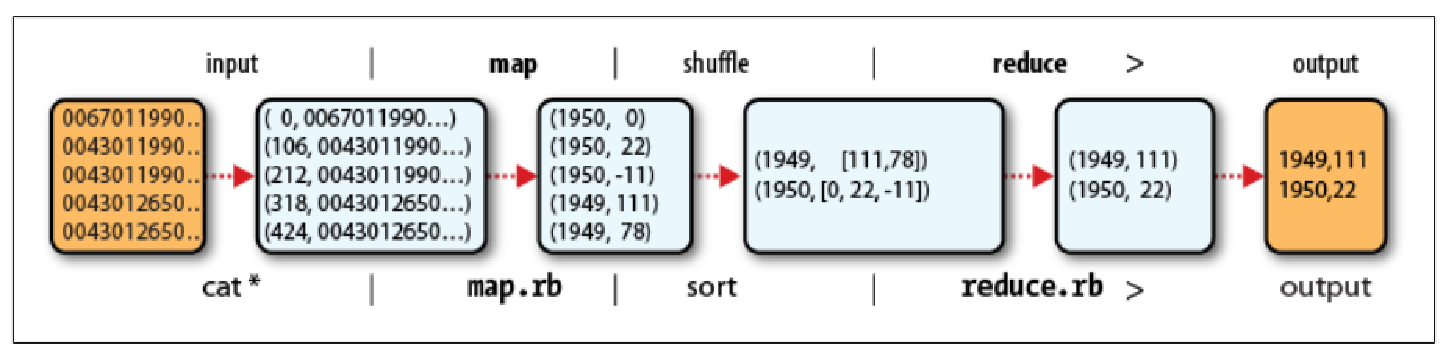
\includegraphics[width=\textwidth,height=\textheight,keepaspectratio]{./Figures/map-reduce.pdf}
    \rule{35em}{0.5pt}
  \caption{MapReduce logical data flow \cite{tom3}}
  \label{fig:map-reduce}
\end{figure}
%\end{verbatim}


\section{ Hadoop}

Hadoop was created by Doug Cutting, the creator of Apache Lucene, the widely used text search library[3].The name hadoop is not an acronyme; it is made-up name by kid of Doug Cutting calling his yellow elephant toy “hadoop”.


Job: MapReduce job is unit of work that need to be processed by nodes. It consist of input data, job configuration information and MapReduce program. To run the jobs, Hadoop divides it into smaller pieces called tasks. There are two types of tasks: map tasks and reduce tasks.

Job execution are controlled by two components of Hadoop called JobTracker and TaskTracker. Jobtracker is responsible to run all jobs on system. It coordinates job execution by scheduling tasks on tasktracker. The jobtracker maintains record about status of each job. The tasktracker executes tasks on nodes and sends progress report to jobtracker. In case if task execution failed, the jobtracker can rescheduler the task on same or different tasktracker.  

Job Creation: Usually the data to be process by Hadoop is very large data set. Hadoop divides this large input data to small fixed-size "input split” or “split”. Each split is called MapReduce job. The splits are fed as input to user defined map function. Map functions read each record of input split and process it. Having many small jobs mean that the execution time for each job is smaller comparing to large input. So if we run the small jobs in parallel on Hadoop cluster, the total time of processing all small jobs will be smaller than total time to process large input data set. 

If the job size is very small , then the job creation and map creation time will dominante the over all execution of job. Therefore usually the size of MapReduce jobs are the same as the HDFS block size , which is 64 MB. Such job size is good for Rack Locality Feature of Hadoop.


\subsection{Hadoop Distributed File System (HDFS)}

HDFS is the file system component of Hadoop which stores large data sets across cluster of computers in reliable and distributed manner. HDFS is designed to stream data in high bandwidth to user applications.
“HDFS is a filesystem designed for storing very large files with streaming data access patterns, running on clusters of commodity hardware” \cite{tom3} \cite{sailfish}.

\textbf{Very Large Files} 
  The “very large” in this context refers to files in size of hundreds of gigabytes or terabytes.

\textbf{Streaming Data}
  The efficient data processing idea behind HDFS design was based on write-once and read many times. Usually data set is generated or copied from source and performance evaluation is executed on large proportion, if not all, of data set. Therefore it is the time to read the whole file is more important than reading the first record\cite{tom3}. 
  
%\subsection{Common \LaTeX{} Math Symbols}
\textbf{Commodity Computers}
   HDFS does not require expensive high-available and reliable hardware. It is designed to run over cluster of  “commonly available hardware from multiple vendors” or so called commodity hardware where the  failure chances of hardware is very high. For case of hardware, HDFS is designed to continue process and work without noticing the user application from hardware failure. HDFS will not work so well for low latency applications and small file.\cite{tom3} 

\textbf{Low-latency data access}
As mentioned earlier HDFS was designed for high throughput of data, loading files may lead to delay. Thus, applications that requires low latency in tens of milliseconds, will not work well using HDFS.\cite{tom3} 

\textbf{Lots of small data}
The inode data and list of blocks belonging to each file is called metadata. The namenode stores the filesystem metadata in random access memory (RAM) [2]. The number of files in namenode is limited by memory size. Each file, directory, and block takes 150 bytes in memory, so, it is feasible to have millions of files, but billions is beyond the capacity of this hardware.\cite{tom3}
   
\subsection{HDFS Blocks}
 
The minimum amount data or sequence of bytes (or bits) that disk can read or write is called disk block size. The size of disk block is usually 530 Bytes [1]. To read and write data into blocks, filesystem blocks which are in size of kilo bytes are created on top of disk blocks. Generally, the disk blocks are transparent to filesystem. 
HDFS also has the concept of block; it is default block size is 64 megabyte. The size of HDFS block can be modified to larger number for example 128 megabytes or 512 megabytes. HDFS breaks the large file into fixed size chunks called HDFS blocks. Each block is stored independently in the cluster. For small file chunks, full capacity of HDFS is not occupied by HDFS. 
The time to read and write on disk depends on two factors called seek time and data transfer rate of the disk. The time needed to move HEAD (data reader or write component of disk) to the block from where it should read or write is called seek time. The amount of data that disk can read and transfer in second is called disk transfer rate which is usually calculated as megabytes per second. HDFS blocks are large compared to disk block size, this is to reduce the seek time of the disk. For large blocks, the data transfer time is significantly bigger compared to seek time to move to beginning of the block, thus time to transfer multiple files is equal to disk transfer rate.
It is not necessary that all blocks of the file to be placed on same single disk.  So, an advantage of the block structure is that if a file is larger than available capacity of single disk in the cluster, it can be stored across multiple disks in the cluster. 

%----------------------------------------------------------------------------------------


\subsection{Namenode and Datanode}

As explained in \cite{tom3}, Hadoop cluster consist of two types of nodes which operates in master-worker pattern: a name-node (the master)and number of datanodes (workers).The namenode is responsible to store and manage filesystem namespace and the metadata for all files and directories in the tree. The information is stored in local disk in two different files "namespace image" and "edit log".The namenode knows all the datanodes on which the blocks for a given file is located.The namenode or clients use datanodes as computational resource and storage for data blocks. Datanodes are workhorses that stores and retrives data when they are told. The datanodes updates the namenode with list of data blocks that they are storing. All the nodes are connected and communicate with each other using TCP-based protocols. The namenode stores copy of data across multiple Data Nodes in the cluster to ensure reliability.

All the information about filesystem is stored on namenode. In case, if namenode data is erased ( due to failure or any other reason), then, all the files on file system is lost because there is no way of how to reconstruct data blocks. There for , having resilient namenode to failure and Hadoop provides two mechanism for this.  

The first way is to configure Hadoop in a way that it write the steady state of the namenode to multiple filesystems as back up copy. The writes are atomic operations that can write to local disk and to a remote NFS(Network File System) mount.

As second solution, it is possible to run another namenode as scondry namenode to merge the imagespace image with edit logs in order to prevent edit log files from becoming to large. Since secondry namenode requires so much CPU and as much memory as namenode, usually, it runs on separate physical machine.The secondry namenode keeps copy of the merged namespace image , and this copy can be used in case of namenode failure. Usually, when namenode fails, copy of namenode data which are on NFS is copied to secondary namenode and runs secondary namenode as new primary.

   


%----- Data -----
%Hadoop stores meta-data and application data separately. The Meta data is stored in server machine so called Name Node. The user %application data is stored on other servers so called Data Node(s).  The advantage of this strategy is that data transfer is %multiplied and there are more chances to locate computation near the data (Data Locality)\cite{sailfish}.




%----------------------------------------------------------------------------------------

%\section{Hadoop Schedulers}

\section{Hadoop Optimizations}

 The optimization relevant to hadoop scheduler is covered in this section.As explained in section one of this chapter, hadoop use mechanism to distribute across cluster of computers. Hadoop use scheduler to assign the jobs to datanodes, thus scheduler has key rule in hadoop's performance.  Many literature suggested approaches to optimize hadoop scheduler performance.
 
 \subsection{Capacity Scheduler}
 
Though organizations can have their own private compute resources with sufficient capacity to execute jobs on, but such private resources may cost expensive and lead to low utilization of resources.Capacity Scheduler is pluggable MapReduce scheduler that is designed to allow multiple-tenants to share large Hadoop cluster securely and to maximize utilization of the cluster.It is cost effective for the organization to share clusters and run jobs comparing to having their own private cluster. 

 Using capacity scheduler , the organizations fund the Hadoop cluster collectively, and obtains their share.The available resource in the Hadoop cluster is partitioned and  guaranteed  minimum share for each organization is provided. In addition, organization can access more then limited share only when the cluster resource is not used by other organization. This mechanism provides elasticity for organization and maximizes the cluster utilization. It means, if other organizations does not use the cluster, then any organization can use full cluster resources(not limited minimum) for its computational jobs as long as their only one organization submitting jobs to the cluster.
 
 As the cluster is shared among organization, this leads to strong cooporation for multi-tenancy to guarantee minimum limit of each organization. To avoid more then limit consume of resources  by single job or user that affects other organization's share, capacity scheduler provides safe-guards that limits the user or job access to its share.The capacity scheduler , manages users and jobs in queue structures and resource share is provided to each queue based on their economical share of the cluster. Typically the queues are setup by administrator.
 
 As mentioned in above paragraph, capacity scheduler is pluggable Hadoop mapreduce job scheduler which is available as JAR file in the hadoop tarball under contrib/ capacity-scheduler directory.It is also possible to build scheduler from source by executing ant package, and source package is available under build/contrib/capacity-scheduler
 
   

 
 
 \subsubsection*{Features}
 \textbf{Capacity Guarantee}

Capacity scheduler supports multiple queues,the organization submit jobs to their relevant queue(s). The cluster resources is allocated between all the queues based on their economical share of the cluster. It mean that certain capacity of the cluster at disposal of jobs of its queue. There could be soft or hard limit between queues configured by administrator. Where soft limit means that queue can access more then limited capacity if the others does not use the resource. Hard limit refers to situation where organization can use only their own share of the resource not more. 


 
 \textbf{Security}
 
In order to prevent unauthorized user to submit jobs to queue, strict access control lists are applied to each queue. The safe-guards can be used to ensure that users can not view or modify jobs from other users.   
 

\textbf{Elasticity } 

It is not must for queue of jobs to use only its share portion of resources.Queues can demand beyond their capacity, if there is chance in future point in tasks, then after scheduled tasks executed and completed on resource, these free resources can be allocated to queue which has demand. This mechanism maximizes resource utilization and ensures that resource are available in elastic manner. 


\textbf{Multi-tenancy }

To ensure that cluster resource is not monopolized by single,job,user and queue limits are provided which ensures that the system or in particular jobTracker is not overwhelmed by too many tasks or jobs. 

\textbf{Operability }

User and administrators can view current allocation of the queues of the system through console. It is also possible to change queue modification during run time without disruption to users. 


\textbf{Resource-based Scheduling }

Resource intensive jobs are those that requires or can demand for higher-requirement then default. Capacity Scheduler can accomodate applications or in particular jobs with different resource requirement. Memory is the only resource currently supported by Capacity Scheduler. 

\textbf{Job Priorities }

Though a running job can not be preempted by any other job, but it is possible to assign higher priority to a job within the queue. Jobs that have higher priority will have access to queue's share of resources faster than jobs with lower priority. By default, priority is disabled in capacity scheduler.\cite{capacity} 


\subsection{Fair-Share Scheduler}

Fair-share scheduler is pluggable mapreduce Hadoop scheduler that maintains separate queues for user groups (pools). Resources are allocated to jobs, in a way that on average every job gets fair share of resources over time. If there is single job running, then, it can utilize full resources of the cluster.For new submitted jobs, the slots that become free will be allocated, this mechanism provides opportunity that each job consume on average roughly same amount of resources. Unlike default Hadoop scheduler that maintain queue of jobs, fair-share scheduler lets short jobs to complete in reasonable time and also it does not starve long jobs.  \cite{dynamic} \cite{fair}

 
The fair-share scheduler maintains jobs into pools, initial fair distribution of resources across multiple pools are assigned to these pools in order to limit their access to resources.In addition to provision of fair share of resources, fair share scheduler can provide minimum guranteed amount of resources( or computer time of CPU) to each pool to ensure that each user,pool gets sufficient amount of resources. If a pool completed its jobs and does not need the resources,excess resources is evenly distributed among other pools.\cite{fair}
 By default there is one queue per user so that all users can get equally same fraction of total resources.The setup of job pool is possible based on Unix user groups or any other jobconf property.Within each queue, jobs can be scheduled as first-in-first-out (FIFO) or fair share schedule. Fair-share can support job priority, where priority is weight that identifies fraction of total compute time for each job. In addition,  inter-queue job priority is also supported by fair-share scheduler.\cite{fair}
 
 
 \textbf{Task Preeption}
 
 In case if minimum share of a pool is not provided, after waiting for certain period of time, the scheduler may kill a task from other pool(s) to provide minimum share to pool.Killing task of other jobs is called task preemption.It is also possible that preemption happen if a pool is below its half share for configurable timeout period.Usually timeout value is higher than minimum share timeout preemption.\cite{fair} \cite{fairw} 
 
In both cases of above preemption , the fair share scheduler kills most-recently-launched tasks from over-allocated jobs, to minimize wasted computation.Since Hadoop jobs are tolerated to losing tasks, killing tasks does not cause jobs to fail but causes them to take longer to finish.\cite{fair}\cite{fairw} 
 














\subsection{Speculative Execution}

The goal of speculative execution is to reduce the job completion time by speculating the tasks from straggler machines. The tasks are categorized into below 3 categories. If there is free slot on a node, then a task is selected according to the category number from one these categories.  

1 - Failed Tasks: If a task fails multiple time , due to a bug and stop the job, such task is marked as "failed task" and given highest priority. 

2 - Non-Running Tasks:These are fresh tasks that has not being executed on any node yet. For maps, data-locality is considered and tasks that are closer to the node is performed first. 

3 - Speculative Tasks:To find speculative task,the progress of task is monitored by hadoop with a progress score between 0 and 1.Map progress depends on input data read and its progress score is fraction of input read data. The reduce phase compromise three sub phases where each sub-phase is counted as 1/3 of progress report. The three sub-phase of reduce phase is explained as a,b,c bullet points bellow. 

	a - Fetching of map outputs, also called copy phase.
	b - Sorting of map outputs by key, also called sort phase.
	c - Applying user-defined function to the list of map outputs with each key, also called reduce phase. 

In each sub-phase of reduce, the score is fraction of data processed. For example, a task halfway through the copy phase has a progress score of 1/2 * 1/3 = 1/6 , while a task halfway through the reduce phase scores 1/3 + 1/3 +(1/2 * 1/3)= 5/6.

\textbf{Straggler} 

For map tasks and reduce tasks average of their progress score is defined as threshold by hadoop.If progress score for a task is less then the the threshold of its category (maps or reduces) minus 0.2, and it has run for at least 2 minutes , it is marked as straggler. All the tasks \b{below,beyond?} the threshold are considered as slow and the scheduler runs at least one speculative copy of these tasks at time. 
 

\textbf{source:Improving MapReduce Performance in Heterogeneous Environments
Matei Zaharia, page:31 on the document}


%%%%%%%%%%%%%%%%%%%%%%%%%%%%%%%%%%%%%%%%%%%%%%%%%%%%%%%%%%%%%%%%%%%%%%%%%%%%%%%%%%
%%%%%%%%%%%%%%%%%%%%%%%%%%%%%%%%%%%%%%%%%%%%%%%%%%%%%%%%%%%%%%%%%%%%%%%%%%%%%%%%%%

\subsection{LATE Scheduler}

"Hadoop’s scheduler can cause severe performance degradation in heterogeneous environments. We design a new scheduling algorithm, Longest Approximate Time to End (LATE), that is highly robust to heterogeneity. LATE can improve Hadoop response times by a factor of 2 in clusters of 200 virtual machines on EC2"[source:Improving mapreduce ...].
LATE is another speculative task scheduler that behave well in real environment[source:Improving mapreduce ...].The task's finish time is estimated and for those tasks that are believed to finish farthest time into the future are speculatively executed. Because the speculative copy are execute in faster nodes so they have better chance to overtake the original copy and reduce job response time. 
The heuristic to estimate time left for task completion is as follow: The \i{progress rate} for each task is estimated as  ProgressScore/T, where T is the amount of time task has been running for. Based on \i{progress rate} the time to completion is estimated as (1 - ProgressScore/ProgressRate). The assumption in this estimation is that task has the same progress rate.
The execution of speculative tasks on fast nodes provides better opportunity that a speculative copy of task overtake the original task. Nodes that are below SlowNodeThreshold are considered as fast nodes and speculative tasks can only be executed on fast nodes no stragglers.Sum of progress scores for all succeded and in progress tasks on the cluster is estimated as speed, and SlowNodeThreshold is defined as percentile of speed below which node will be considered as slow node.This avoids unnecessary speculation when only fast tasks are running.  
The total number of speculative tasks that can be executed in one time, is defined as \i{SpeculativeCap}.If less then SpeculativeCap speculative is running, and an free node asks for task then the task assignment decision is made as follow:
 - If node is slow(total progress is lower than SlowNodeThreshold) then ignore the request. 
 - Estimate the time left for running tasks that are not speculated and rank them for speculative execution. 
 - Run the copy of task with highest rank (lowest progress rate comparing to SlowTaskThreshold). 
 
"In practice, we have found that a good choice for the three parameters to LATE are to set the SpeculativeCap to 10\% percent of available task slots and set the SlowNode- Threshold and SlowTaskThreshold to the 25th percentile of node progress and task progress rates respectively [source matie zahrie]."
 
\subsection{Advantages of LATE}

The native Hadoop scheduler mechanism is to consider any task that is below the fixed threshold as slow task and treat them equally for speculative execution. While, LATE relaunches the slowest task and small number(at maximum as SpeculativeCap) of tasks to limit contention for shared resources.LATE mechanism is to prioritize among slow tasks on how much they hurt job response time and rank them for speculation priority.
Hadoop native scheduler assumes that nodes are homogeneous and any candidate node for task execution is likely to be a fast node. In contrast, LATE takes into account node heterogeneity by ranking some nodes as slow node(nodes below SlowNodeThreshold are marked as slow node)and assigns new tasks only to fast nodes.
Hadoop native scheduler focuses on progress rate and speculativly executes any slow task.LATE focuses on estimated time left and speculatively executes only tasks that will improve job response time. For example,if task A is 5x slower than the mean but has 90 percent progress, and task B is 2x slower than the mean but is only at 10 percent progress, then task B will be chosen for speculation first, even though it is has a higher progress rate, because it hurts the response time more. Therefore , LATE provides opportunity for slow nodes to be utilized as long as this does not hurt job response time which is unlike of progress rate base scheduler that always re-executes task from slow nodes.      


